A participação cidadã e a colaboração em governos eletrônicos (e-Gov) têm se tornado cada vez mais relevantes na sociedade contemporânea. Com o avanço da tecnologia e a disseminação das redes sociais, surgiram novas formas de engajamento e interação entre cidadãos e governos. Nesse contexto, o aplicativo Colab.re desponta como uma plataforma inovadora que combina elementos de redes sociais com a participação cidadã em questões relacionadas à gestão pública. Neste capítulo, exploraremos o Colab.re sob a perspectiva das redes sociais e e-Gov, analisando suas funcionalidades, impactos sociais, desafios e limitações.
\begin{citacao}
    "uma forma de inteligência coletiva em que as pessoas se reúnem para monitorar, analisar e agir coletivamente em relação a um problema ou questão compartilhada" \cite[p. 1]{2011_Bryer}.
\end{citacao}

\section*{História e Desenvolvimento}
O Colab.re foi lançado em [ano de lançamento] como uma iniciativa pioneira no campo da participação cidadã digital. A plataforma foi desenvolvida com o objetivo de promover a interação entre cidadãos e governos, permitindo que os usuários compartilhem ideias, façam sugestões, denunciem problemas e participem ativamente na construção de políticas públicas. Desde então, o Colab.re tem conquistado espaço em diversas cidades, tornando-se uma ferramenta de referência no campo da democracia digital.

\section{Funcionalidades}

O Colab.re oferece uma variedade de funcionalidades que estimulam a participação cidadã e promovem a interação entre os usuários. Entre as principais funcionalidades do aplicativo, destacam-se:

\begin{itemize}
  \item \textbf{Publicação de ideias e sugestões:} Os usuários podem compartilhar suas ideias e sugestões sobre questões de interesse público. Essas publicações podem abranger diversos temas, desde melhorias na infraestrutura urbana até propostas de políticas sociais.

  \item \textbf{Denúncia de problemas:} O Colab.re permite que os cidadãos denunciem problemas, como buracos nas vias, iluminação pública deficiente, entre outros. Essas denúncias são georreferenciadas, o que facilita a identificação e resolução dos problemas pelas autoridades competentes.

  \item \textbf{Interatividade social:} O aplicativo permite que os usuários sigam outros usuários, sejam seguidos, curtam e comentem as publicações. Essa interatividade promove a formação de uma rede social dentro do Colab.re, ampliando as possibilidades de engajamento e diálogo entre os participantes.

  \item \textbf{Acompanhamento de demandas:} Os usuários podem acompanhar o andamento das demandas e propostas que foram apresentadas. Isso permite que eles estejam cientes das ações tomadas pelo governo em resposta às suas contribuições.
\end{itemize}

Através dessas funcionalidades, o Colab.re busca fortalecer a participação cidadã e criar um ambiente propício para o diálogo entre cidadãos e governos. Além disso, o aplicativo também oferece uma série de benefícios para os usuários, como a possibilidade de influenciar diretamente as políticas públicas e a oportunidade de se conectar com outros cidadãos que compartilham os mesmos interesses.

\section{Plataformas de Participação cidadã e e-Gov}
O Colab.re se destaca no cenário das plataformas de participação cidadã devido às suas características específicas. Ao compará-lo com outras plataformas similares, é possível observar algumas diferenças significativas. Por exemplo, enquanto algumas plataformas focam principalmente na coleta de dados e informações dos usuários, o Colab.re se concentra em incentivar a participação ativa e o diálogo entre os cidadãos e os governos. Além disso, o Colab.re se destaca pela sua interface amigável e pela capacidade de georreferenciamento das denúncias, o que permite uma maior eficácia na resolução dos problemas reportados.

\section{Impacto do Colab.re em cidades}
O Colab.re tem demonstrado um impacto significativo nas cidades em que está presente. Por exemplo, em um estudo realizado na cidade de Paragominas-PA, o aplicativo foi utilizado como um dispositivo de participação social na gestão urbana, permitindo que os cidadãos reportassem problemas e propusessem soluções [1]. O estudo constatou que o Colab.re contribuiu para uma maior transparência e eficácia na resolução dos problemas urbanos, além de fortalecer o engajamento cívico na cidade.

Além de Paragominas, o Colab.re também tem sido adotado em outras cidades brasileiras, como São Paulo, Rio de Janeiro e Fortaleza. Através da plataforma, os cidadãos têm a oportunidade de participar ativamente na gestão pública, compartilhando suas opiniões, denunciando problemas e colaborando na construção de uma cidade mais inclusiva e sustentável.

\section{Estudos de caso do Colab.re na resolução de problemas urbanos}
O Colab.re tem sido utilizado em diversos casos para resolver problemas específicos e melhorar a qualidade de vida nas cidades. Por exemplo, em um estudo de visualização de dados em aplicativos móveis, o Colab.re foi investigado como um exemplo de aplicativo de cidade inteligente [2]. O estudo mostrou que o aplicativo oferece recursos de visualização de dados que permitem aos usuários entender melhor os problemas urbanos e contribuir de forma mais efetiva para a sua resolução.

Outro estudo relatou o caso de um aplicativo que utilizou o Colab.re como plataforma para denúncias de problemas relacionados ao sistema de informações geográficas (GIS) e colaboração coletiva [3]. O estudo destacou a eficácia do Colab.re na coleta de dados georreferenciados e no engajamento dos cidadãos na solução de problemas urbanos.

Esses estudos de caso demonstram como o Colab.re tem sido usado de forma efetiva para resolver problemas específicos e melhorar a qualidade de vida nas cidades.

\section{Dados}

Com base nos dados disponibilizados pelo Colab para esse estudo, analisamos um total de 328.876 eventos criados entre 04/01/2013 e 05/12/2022. Para essa análise foi utilizado a linguagem Python e a biblioteca Pandas. O código fonte está disponível no GitHub.

\subsection{Modelo de dados}

\begin{table}[ht]
    \centering
    \caption{Modelo de Dados da lista de usuários}
    \label{tab:user_model}
    \begin{tabular}{|l|p{6cm}|}
    \hline
    \textbf{Campo} & \textbf{Descrição} \\
    \hline
    colab\_user\_id & Identificador único do usuário no sistema Colab \\
    gender & Gênero do usuário \\
    birth\_date & Data de nascimento do usuário \\
    city\_id & Identificador único da cidade do usuário \\
    city\_name & Nome da cidade do usuário \\
    state\_id & Identificador único do estado do usuário \\
    state\_name & Nome do estado do usuário \\
    created\_at & Data de criação do registro do usuário \\
    last\_sign\_in\_at & Data da última vez que o usuário fez login \\
    device & Dispositivo utilizado pelo usuário (por exemplo, desktop, mobile) \\
    \hline
    \end{tabular}
\end{table}

\begin{table}[ht]
    \centering
    \caption{Modelo de Dados de eventos reportados}
    \label{tab:event_model}
    \begin{tabular}{|l|p{6cm}|}
    \hline
    \textbf{Campo} & \textbf{Descrição} \\
    \hline
    event\_id & Identificador único do evento \\
    user\_id & Identificador único do usuário relacionado ao evento \\
    description & Descrição do evento \\
    status & Status do evento \\
    created\_at & Data de criação do evento \\
    event\_type\_id & Identificador único do tipo de evento \\
    event\_type\_name & Nome do tipo de evento \\
    \hline
    \end{tabular}
\end{table}

Os dados dos foram disponibilizados em formato CSV, contendo informações sobre os usuários e os eventos reportados. A tabela \autoref{tab:user_model} apresenta o modelo de dados da lista de usuários. A tabela \autoref{tab:event_model} apresenta o modelo de dados de eventos reportados.

\subsection{Distribuição demográfica}

O quadro \autoref{quadro:usersbygender} apresenta a distribuição demográfica dos usuários por gênero. A maioria dos usuários se declararam do gênero másculino. 


\begin{quadro}[htb]
    \caption{Usuários por gênero}
    \label{quadro:usersbygender}
    \centering
    \pie[
            % Opções de aparência do gráfico
            radius=2.5, % Raio do gráfico de pizza
            text=pin, % Posição do texto no gráfico
            rotate=90 % Rotação do gráfico
        ]{
            30494/Masculino,
            19555/Feminino,
            16/Não Binário,
            335/Desconhecido,
            274/Outro,
            92/Não Informado
        }
\end{quadro}

\subsection{Tipos de Eventos}

\begin{table}[h]
    \centering
    \caption{Tipos de eventos com mais ocorrências}
    \label{tab:tiposevento}
    \begin{tabular}{|l|l|l|}
    \hline
    \textbf{Tipo de Evento} & \textbf{Total de Ocorrências} \\
    \hline
    Entulho na calçada/via pública            & 61.785 \\
    Buraco nas vias                           & 41.200 \\
    Lâmpada apagada à noite                   & 32.907 \\
    Ponto de infração de trânsito recorrente  & 15.873 \\
    Calçada irregular                         & 14.837 \\
    Mato alto                                 & 13.459 \\
    Poda de árvore                            & 12.810 \\
    Descarte irregular de lixo                & 12.685 \\
    Bueiro entupido                           & 8.825  \\
    Vazamento de água                         & 7.433  \\
    Bueiro sem tampa                          & 5.844  \\
    Ocupação irregular de área pública        & 5.714  \\
    Fiação irregular                          & 5.643  \\
    Veículo abandonado                        & 5.335  \\
    Equipamento público danificado            & 4.694  \\
    Esgoto a céu aberto                       & 4.656  \\
    Retirada de árvore                        & 4.437  \\
    Ponto recorrente de poluição sonora       & 4.189  \\
    Bloqueio na via                           & 4.066  \\
    Iluminação pública irregular              & 3.702  \\
    \hline
    \end{tabular}
\end{table}

A tabela \autoref{tab:tiposevento} apresenta os 20 tipos de evento mais reportados pelos usuários. A análise dos dados fornecidos pelos usuários do Colab proporcionou insights valiosos sobre as preocupações e demandas da comunidade. Os eventos mais frequentemente relatados estão intrinsecamente ligados a problemas e irregularidades na infraestrutura urbana, como entulho na calçada/via pública, buraco nas vias, lâmpada apagada à noite, ponto de infração de trânsito recorrente e calçada irregular. Essas ocorrências destacam a importância de investimentos contínuos na manutenção e melhoria da infraestrutura da cidade. Além disso, questões ambientais emergem como uma área de preocupação significativa, com denúncias frequentes de descarte irregular de lixo, desmatamento ilegal, esgoto a céu aberto e mato alto. Tais dados indicam uma conscientização dos usuários em relação à preservação ambiental e ressaltam a necessidade de ações efetivas para aprimorar a gestão dos recursos naturais. O transporte público também é alvo de atenção, com reclamações recorrentes sobre problemas em ônibus, atrasos e superlotação. Esses aspectos exigem uma análise aprofundada das questões relacionadas à mobilidade urbana e podem impulsionar esforços para melhorar a qualidade e eficiência do transporte coletivo. Além disso, eventos relacionados à segurança e vigilância, como pontos de exploração sexual de menores e maus-tratos a animais, refletem a preocupação dos usuários com a proteção e bem-estar da comunidade. Por fim, a ocorrência de eventos envolvendo estabelecimentos comerciais, como falta de alvará e condições sanitárias irregulares, destaca a importância de ações rigorosas de fiscalização e de garantir a conformidade legal por parte dos estabelecimentos. Esses insights fornecem uma visão abrangente das preocupações dos usuários do Colab e podem orientar as prefeituras da cidade na implementação de políticas públicas que visem atender às demandas da comunidade e aprimorar a qualidade de vida em geral.

Os usuários estão engajados e ativos na identificação e denúncia de problemas na infraestrutura urbana, meio ambiente, transporte público e questões sociais. Isso indica uma participação cidadã ativa e um desejo de melhorar as condições de suas comunidades.
Os clientes podem aproveitar essas informações para acompanhar as preocupações e demandas da comunidade, tomar medidas corretivas mais efetivas e aprimorar a qualidade dos serviços e infraestrutura oferecidos.

Os dados fornecem uma visão clara das principais questões enfrentadas pela comunidade, permitindo que as prefeituras priorizem recursos e esforços em áreas críticas, como manutenção da infraestrutura, gestão ambiental, transporte público e segurança. As prefeituras podem usar esses insights para desenvolver políticas públicas mais eficazes, implementar medidas preventivas e corretivas, bem como estabelecer canais de comunicação e interação mais robustos com os cidadãos, fortalecendo a confiança e a participação da comunidade nas decisões governamentais.

\begin{figure}[!htb]
    \caption{Histograma demonstrando a distribuição de novos eventos por ano}
    \label{fig:colab_events_overtime}
    \centering
    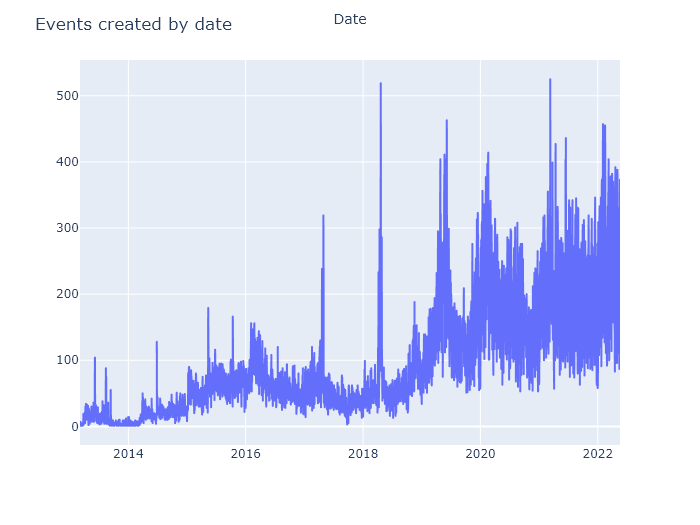
\includegraphics[scale=0.25]{colab_events_overtime.png}
\end{figure}

O gráfico \autoref{fig:colab_events_overtime} demonstra a criação de eventos ao longo dos anos. Na imagem pode-se identificar dois picos de postagens: 2018 e 2022. O primeiro pico pode ser explicado pela popularização do aplicativo, que foi lançado em 2017. Já o segundo pico pode ser explicado pela pandemia de COVID-19, que fez com que as pessoas passassem mais tempo em casa e, consequentemente, observassem mais problemas na infraestrutura urbana.

\section*{O papel do Colab.re na transparência governamental}
A transparência governamental é um elemento essencial para a democracia e o bom funcionamento das instituições públicas. O Colab.re desempenha um papel importante na promoção da transparência, uma vez que todas as denúncias, propostas e ações tomadas pelo governo são visíveis para os usuários da plataforma. Isso permite que os cidadãos acompanhem o andamento das demandas, fiscalizem as ações do governo e tenham acesso às informações sobre a gestão pública. Essa transparência fortalece a confiança e a accountability entre os governantes e os governados.

\section*{Contribuições do Colab.re para a democracia digital}
A democracia digital refere-se à utilização da tecnologia para fortalecer a participação e o engajamento cívico. Nesse contexto, o Colab.re desempenha um papel significativo ao oferecer uma plataforma acessível e interativa para os cidadãos se envolverem na gestão pública. Através do aplicativo, os cidadãos têm a oportunidade de expressar suas opiniões, contribuir com propostas e denunciar problemas, promovendo assim uma participação mais ampla e inclusiva na tomada de decisões.

\section*{Desafios dos usuários do Colab.re}
Apesar dos benefícios e do potencial do Colab.re, há desafios que os usuários podem enfrentar ao utilizar a plataforma. Por exemplo, a falta de conhecimento ou acesso à tecnologia pode limitar a participação de certos grupos de cidadãos. Além disso, a confiança no governo e a percepção de que as contribuições dos cidadãos são levadas em consideração são fatores-chave para incentivar o engajamento contínuo dos usuários.

\section*{Como o Colab.re pode ser melhorado no futuro}
Para garantir a eficácia contínua do Colab.re e maximizar seu potencial, é importante considerar melhorias e atualizações futuras. Algumas sugestões incluem aprimorar a interface do usuário para torná-la mais intuitiva e amigável, expandir a divulgação e o treinamento para aumentar a conscientização e o acesso ao aplicativo, e estabelecer parcerias com outras instituições e organizações para ampliar o impacto e a cobertura do Colab.re.

\section*{O Colab.re e a participação cidadã durante a pandemia de COVID-19}
A pandemia de COVID-19 trouxe desafios sem precedentes para a participação cidadã e o engajamento social. Nesse contexto, o Colab.re desempenhou um papel importante ao permitir que os cidadãos se envolvessem virtualmente na gestão pública, mesmo durante o distanciamento social. Através do aplicativo, os cidadãos puderam denunciar problemas relacionados à pandemia, compartilhar informações relevantes e contribuir com propostas para enfrentar os desafios impostos pela crise sanitária.

\section*{Conclusão}
Em conclusão, o Colab.re representa uma importante ferramenta no contexto das redes sociais e e-Gov. Com suas funcionalidades inovadoras, o aplicativo tem promovido a participação cidadã, fortalecido a transparência governamental e contribuído para a democracia digital. Apesar dos desafios e limitações, o Colab.re demonstra um impacto significativo nas cidades onde é adotado, melhorando a qualidade de vida dos cidadãos e fortalecendo a governança local. À medida que avançamos em direção a um futuro cada vez mais digital, é essencial continuar explorando o potencial do Colab.re e outras plataformas semelhantes para promover uma participação mais inclusiva e engajada dos cidadãos na gestão pública.